\documentclass{article}
\usepackage[utf8]{inputenc}
\usepackage{graphicx}
\usepackage{whilecode2}

\title{Practica 3}
\author{Jose Antonio Guardeño Algar}
\date{December 2022}

\begin{document}

\maketitle
\section{Ejercicio 1}
1. Define the TM solution of exercise 3.4 of the problem list and test its correct
behaviour.

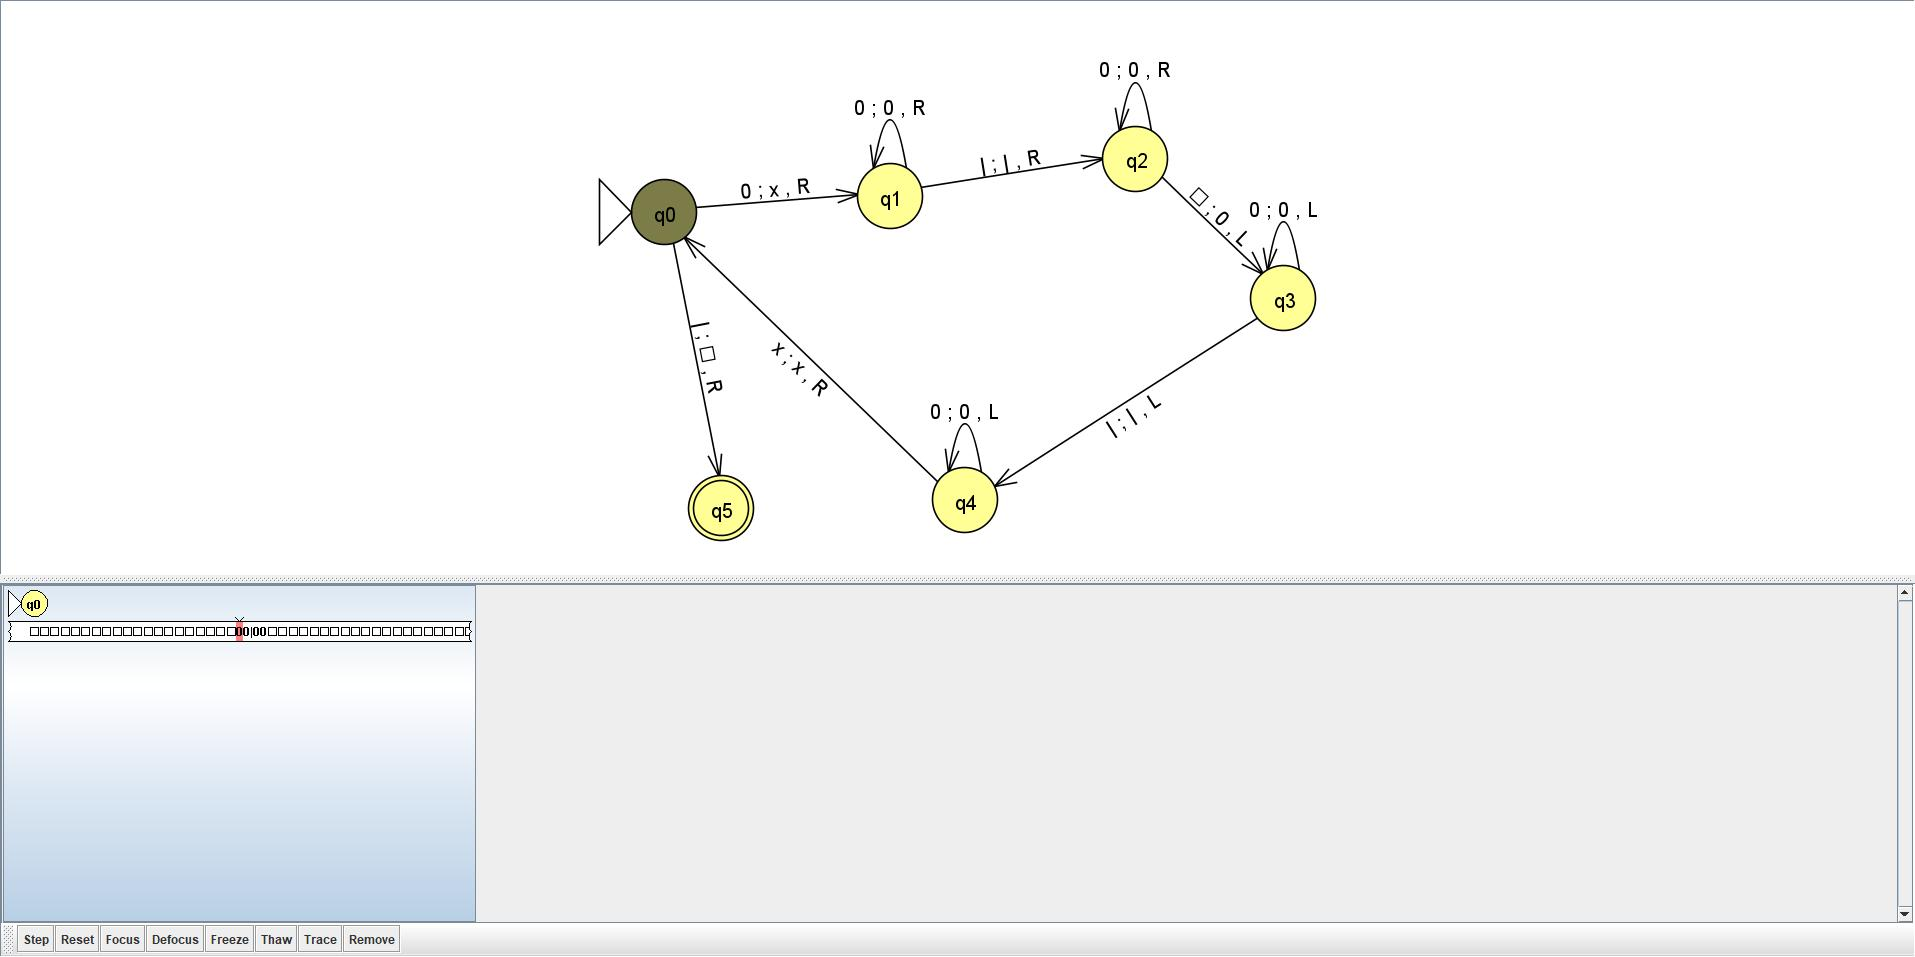
\includegraphics[width=15cm]{Practica31.jpg}
\section{Ejercicio 2}
\newline
2. Define a recursive function for the sum of three values.
\newline
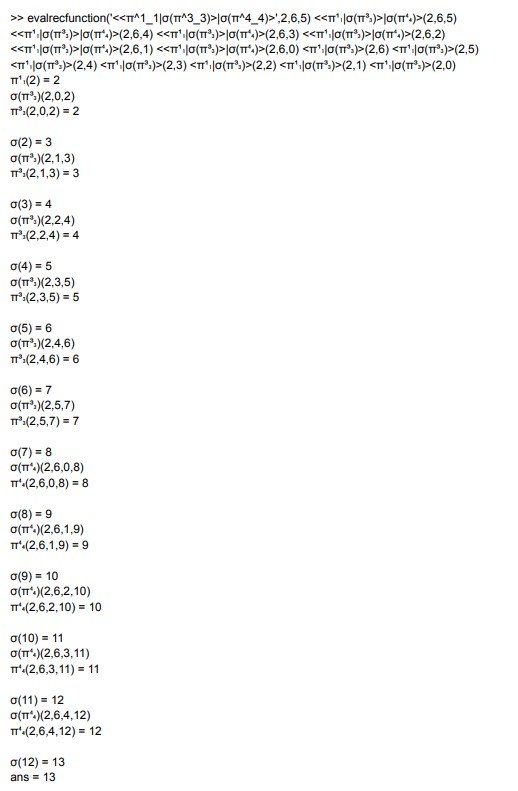
\includegraphics{practica32pd.jpg}
\section{Ejercicio 3}
3. Implement a WHILE program that computes the sum of three values. You
must use an auxiliary variable that accumulates the result of the sum.
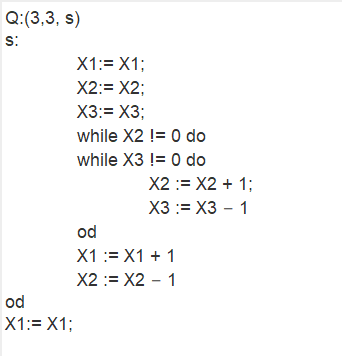
\includegraphics{imagen_2022-12-26_154006801.png}

\end{document}
